\chapter{Conceptos básicos sobre códigos}%
\label{chap:conceptos_básicos_sobre_códigos}

En este capítulo presentaremos los conceptos básicos sobre códigos lineales, para lo cual nos hemos basado casi por completo en el primer capítulo de~\cite{huffman_fundamentals_2003}.

\section{Códigos lineales, matrices generadora y de paridad}%
\label{sec:códigos_lineales_matrices_generadora_y_de_paridad}

Sea \(\F_q\) el cuerpo finito de \(q\) elementos y \(\F_q^n\) el espacio vectorial de todas las \(n\)-tuplas sobre dicho cuerpo.

\begin{definition}[Código lineal]
Si \(\mathcal{C}\) es un subespacio vectorial de dimensión \(k\) de \(\F_q^n\), diremos que \(\mathcal{C}\) es un \([n,k]\) \textit{código lineal} sobre \(\F_q\).
\end{definition}

Normalmente escribiremos los vectores \((a_1, a_2, \dots, a_n)\) en \(\F_q^n\) de la forma \(a_1 a_2 \cdots a_n\) y llamaremos a los vectores en \(\mathcal{C}\) \textit{palabras código}. Además, utilizaremos nombres concretos para referirnos a códigos sobre algunos de los cuerpos más comunes. A los códigos sobre \(\F_2\) los llamaremos \textit{códigos binarios}, los códigos sobre \(\F_3\) los notaremos como \textit{códigos ternarios} y a los códigos sobre \(\F_4\) los llamaremos \textit{códigos cuaternarios}.\\

Dicho esto, las dos maneras más comunes de presentar un código lineal son dando una matriz generadora o una matriz de paridad.

\begin{definition}[Matriz generadora]
    Una \textit{matriz generadora} de un \([n,k]\) código lineal \(\mathcal{C}\) es cualquier matriz \(G\) de dimensiones \(k \times n\) cuyas filas formen una base de \(\mathcal{C}\).
\end{definition}

Dada una matriz generadora \(G\), para cualquier conjunto de \(k\) columnas independientes de esta, diremos que el correspondiente conjunto de coordenadas o posiciones es un \textit{conjunto de información} de C. Las restantes \(r=n-k\) coordenadas las notaremos como \textit{conjunto de redundancia}, y llamaremos a \(r\) \textit{redundancia} de \(\C\). Si las primeras \(k\) coordenadas forman un conjunto de información, existe una única matriz generadora para el código de la forma \([I_k | A]\) donde \(I_k\) es la matriz identidad de orden \(k\). Diremos que una matriz generadora así está en \textit{forma estándar}.

\begin{definition}
    Una \textit{matriz de paridad } de un \([n,k]\) código lineal \(\C\) es cualquier matriz \(H\) de dimensiones \((n-k)\times n\) tal que
    \[
    \C = \{x \in \F_q^n | Hx^T = 0\}
    .\]
\end{definition}

Como un código lineal es un subespacio de un espacio vectorial, es el núcleo de alguna aplicación lineal, y por tanto, para un código lineal siempre existe alguna matriz de paridad \(H\). Mencionemos que las filas de \(H\) son también independientes. Esto es porque, \(H\) es una aplicación lineal de \(\F_q^n\) en  \(\F_q^{n-k}\), y el núcleo de dicha aplicación lineal es \(\C\) que ya dijimos que tiene dimensión \(k\), por tanto la dimensión de la imagen de la aplicación lineal dada por \(H\) es \(n-k\) y así el rango de \(H\) también es \(n-k\).

\section{Pesos y distancias}
La característica que distingue un código lineal de un mero subespacio vectorial es la distancia. En realidad, un código lineal debería definirse como un subespacio vectorial de un espacio vectorial dotado de una distancia. Aunque no las tratemos aquí, hay otras distancias, como la del rango, que se usan. De esta manera, el mismo subespacio vectorial puede considerarse como dos códigos distintos.

\begin{definition}
Dados dos vectores \(x, y \in \F_q^n\), definimos la distancia \textit{Hamming} entre ellos \(d(x,y)\) como el numero de coordenadas en las que  \(x\) e \(y\) difieren.
\end{definition}

Veamos que en efecto esta es una distancia:

\begin{proposition}
\label{prop:distance}
La función distancia \(d(x,y)\) satisface las siguientes condiciones:
\begin{enumerate}
    \item \(d(x,y) \geq 0\) para todo \(x, y \in \F_q^n\).
    \item \(d(x,y) = 0\) si y solo si \(x = y\).
    \item \(d(x,y) = d(y,x)\) para todo \(x,y \in \F_q^n\)
    \item \(d(x,z) \leq d(x,y) + d(y,z)\) para todo \(x, y, z \in \F_q^n\)
\end{enumerate}

\begin{proof}
Las tres primeras propiedades se comprueban directamente por la propia definición de \(d\). Veamos pues la demostración de la propiedad 4.

Dados dos vectores \(x, y \in \F_q^n\), definimos el conjunto \(D(x,y) = \{i | x_i \neq y_i\}\), y denotamos el complementario por \(D^c(x, y) = \{i | x_i = y_i\}\). Es claro que entonces el cardinal de \(D(x,y)\) coincide con nuestra distancia.

Recordemos también algunas propiedades sobre cardinales de conjuntos que nos serán útiles para terminar la prueba. Sea un conjunto \(A\), notemos por \(|A|\) su cardinal. Entonces, para cualesquiera conjuntos \(A\) y \(B\):
\begin{enumerate}
    \item \(|A| \leq |A \cup B|\)
    \item \(|A \cup B| \leq |A| + |B|\)
    \item Si \(|A| \leq |B|\), entonces \(|A^c| \geq |B^c|\)
\end{enumerate}
Con esto, dados \(x, y, z \in \F_q^n\), conjuntos tenemos que

\[
D^c(x,z) = \{i | x_i = z_i\} = \{i | x_i = z_i = y_i\} \cup \{i | x_i = z_i \neq y_i\}
\]
\[
\implies |D^c(x,z)| \geq |\{i | x_i = z_i = y_i\}| = |\{i | x_i = y_i\} \cap \{i | z_i = y_i\}|
\]
\[
\implies |D(x,z)| \leq |\{i | x_i \neq y_i\} \cup \{i | z_i \neq y_i\}| = |D(x,y) \cup D(y,z)|
\]
\[
\implies |D(x,z)| \leq |D(x,y)| + |D(y,z)|
\]
quedando demostrado el resultado.
\end{proof}
\end{proposition}

Ahora, la \textit{distancia (mínima)} de un código \(\C\) es la mínima distancia entre dos palabras distintas de dicho código. Esta propiedad será crucial a la hora de determinar el número de errores que podrá corregir un código.

\begin{definition}
Diremos que el peso (\textit{de Hamming}) \(wt(x)\) de un vector \(x \in \F_q^n\) es el número de coordenadas distintas de cero de \(x\).
\end{definition}

Si tenemos dos vectores \(x, y \in \F_q^n\) es inmediato comprobar que \(d(x,y) = wt(x - y)\). En el siguiente resultado mostramos la relación entre las propiedades de distancia y peso.

\begin{proposition}
Si \(\C\) es un  código lineal, la distancia mínima coincide con el mínimo de los pesos de las palabras distintas de cero de \(\C\).

\begin{proof}
Sea \(\delta = d(x,y)\) la distancia mínima del código \(\C\), que se alcanza entre dos vectores \(x, y \in \C\), y \(\omega = wt(z)\) el peso mínimo que se alcanza en un elemento \(z \in C\). Sabemos que \(x, y \) y \(z\) existen pues el conjunto de distancias posibles es finito.

Por ser \(\C\) un subespacio vectorial,  \(0 \in \C\), y por tanto  \(\delta \leq d(z, 0) = wt(z) = \omega\). De nuevo por ser \(\C\) un subespacio vectorial tenemos que \(x-y \in \C\), luego \(\omega \leq wt(x-y) = d(x,y) = \delta\), de donde \(\delta = \omega\).
\end{proof}
\end{proposition}

Como consecuencia de este resultado, para códigos lineales, a la distancia mínima también se la llama \textit{peso mínimo} del código. En adelante, si el peso mínimo \(d\) de un \([n,k]\) código es conocido, entonces nos referiremos al código como un \([n,k,d]\) código.

A continuación mostramos que existe una relación elemental entre el peso de una palabra y una matriz de paridad de un código lineal.

\begin{proposition}
    Sea \(\C\) un código lineal con matriz de paridad \(H\), y \(c \in \C\) una palabra de dicho código. Entonces, las columnas de \(H\) que corresponden a coordenadas no nulas de \(c\) son linealmente dependientes. En el sentido contrario, si existe una dependencia lineal con coeficientes no nulos entre \(\w\) columnas de  \(H\), entonces existe una palabra en \(\C\) de peso \(w\) cuyas coordenadas no nulas corresponden a dichas columnas.
\end{proposition}

\begin{proof}
    Sea \(c = (c_1, c_2, \dots, c_n) \in \C\), \(J \subset \{1, 2, \dots, n\}\) tal que \(c_j \neq 0\) si y solo si \(j \in J\). Entonces, por ser \(H\) una matriz de paridad de \(\C\) tenemos que
    \[
    Hc^T = 0,
    \]
es decir, si \(H = (h_{ij})\) con \(i \in \{1,\dots, n-k\}, j \in \{1,\dots, n\}\),
\[
Hc^T =
\begin{pmatrix}
   \sum_{j=1}^n h_{1j} c_j \\
   \sum_{j=1}^n h_{2j} c_j \\
    \vdots \\
   \sum_{j=1}^n h_{(n-k)j} c_j
\end{pmatrix}
= \sum_{j=1}^n c_j
\begin{pmatrix}
    h_{1j}\\
    h_{2j}\\
    \vdots \\
    h_{(n-k)j}
\end{pmatrix}
= \sum_{j\in J} c_j
\begin{pmatrix}
    h_{1j}\\
    h_{2j}\\
    \vdots \\
    h_{(n-k)j}
\end{pmatrix}
= 0
\]
quedando demostrada la primera parte.

Por otro lado, dado \(J = \{j_1, \dots, j_w\} \subset \{1, \dots, n\}\), supongamos que tenemos una dependencia lineal entre las columnas asociadas a \(J\) dada por \(c_{j_1}h_{i j_1} + \cdots + c_{j_w} h_{i j_w}\) para cualquier \(i = 1, \dots, n-k\). Entonces, si construimos \(c = (c_1, \dots, c_n) \in \F_q^n\) como sigue
\[
\begin{cases}
    c_j = 0 & \text{si } j \not \in J \\
    c_j = c_{j_l} & \text{si } j = j_l \in J
\end{cases}
,\]

es evidente que \(wt(c) = w\), y que
\[
Hc^T = \sum_{j \in J} c_j
\begin{pmatrix}
    h_{1j}\\
    h_{2j}\\
    \vdots \\
    h_{(n-k)j}
\end{pmatrix} = 0
\]
terminando la demostración de la proposición.
\end{proof}

Una manera de encontrar la distancia mínima \(d\) de un código lineal es examinar todas las palabras no nulas. El siguiente corolario, que es consecuencia directa de la proposición recién demostrada, muestra como utilizar una matriz de paridad para hallar \(d\).

\begin{corollary}
\label{cor:distance_parity_matrix}
Un código lineal tiene peso o distancia mínima \(d\) si y solo si su matriz de paridad tiene un conjunto de \(d\) columnas linealmente dependientes pero ninguno de \(d-1\) columnas linealmente dependientes.
\end{corollary}

\section{Codificar y decodificar}

\subsection{Codificar}%
Sea \(\C\) un \([n,k]\) código lineal sobre el cuerpo \(\F_q\) con matriz generadora \(G\). Como este es un subespacio vectorial de \(\F_q^n\) de dimensión \(k\), contiene \(q^k\) palabras, que están en correspondencia uno a uno con \(q^k\) posibles mensajes. Por esto, la forma más simple es ver estos mensajes como \(k\)-tuplas \(x\) en \(\F_q^k\). Así, lo más común es codificar un mensaje \(x\) como la palabra \(c = xG\). Si G está en forma estándar, las primeras \(k\) coordenadas son los símbolos de información \(x\); el resto de \(n-k\) símbolos son los de paridad, es decir, la redundancia añadida a \(x\) con el fin de poder recuperarla si ocurre algún error. Dicho esto, la matriz \(G\) puede no estar en forma estándar. En particular, si existen índices de columnas \(i_1, i_2, \dots, i_n \) tales que la matriz \(k \times k\) formada por estas columnas es la matriz identidad, entonces el mensaje se encuentra en las coordenadas \(i_1, i_2, \dots, i_n \) separado pero sin modificar, es decir, el símbolo del mensaje \(x_j\) se encuentra en la componente \(i_j\) de la palabra código. Si esto ocurre diremos que el codificador es \textit{sistemático}.

\subsection{Decodificar}%
\label{sub:decodificar_y_el_teorema_de_shannon}

El proceso de decodificar, consistente en determinar qué palabra (y por tanto qué mensaje \(x\)) fue mandado al recibir un vector \(y\), es más complejo. Encontrar algoritmos de decodificación eficientes es una área de investigación muy relevante en la teoría de códigos debido a sus aplicaciones prácticas. En general, codificar es sencillo y decodificar es complicado, especialmente si tiene un tamaño suficientemente grande.

Con la intencion de establecer las bases para decodificar, comenzamos con un posible modelo matemático de un canal transimitiendo información binaria. A este modelo se le llama \textit{canal binario simétrico} (o CBS) con \textit{probabilidad de recombinación} \(\varrho\) y lo mostramos en la figura~\ref{fig:binary_sym_channel}. Si un \(0\) o un \(1\) son mandados por el canal, la probabilidad de recibirlo sin errores es \(1 - \varrho\); si un \(0\) (respectivamente un \(1\)) son mandados, la probabilidad de recibir un \(1\) (o un \(0\) respectivamente) es \(\varrho\). En la mayoría de casos prácticos \(\varrho\) es muy pequeña. Esto es un ejemplo de un \textit{canal discreto sin memoria} (o CDM), es decir, un canal en el que la salida y la entrada son discretos y la probabilidad de error en un bit es independiente de los bits anteriores en caso de existir. Asumiremos que lo normal sea que un bit se reciba sin errores, así que diremos \(\varrho < 1/2\).

\begin{figure}[h]
    \centering
    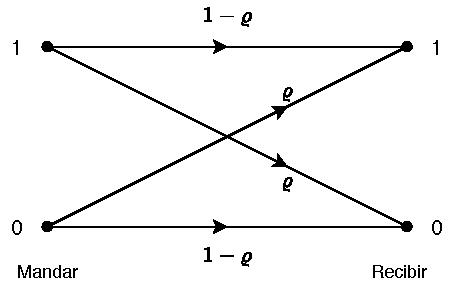
\includegraphics[width=0.4\textwidth]{diagram.pdf}
    \caption{Canal Binario Simétrico}
    \label{fig:binary_sym_channel}
\end{figure}

Si \(E_1\) y \(E_2\) son dos posibles eventos, denotaremos por \(\prob (E_1)\) la probabilidad de que \(E_1\) ocurra y \(\prob (E_1 \mid E_2)\) la probabilidad de que \(E_1\) ocurra supuesto que \(E_2\) ocurre. Supongamos que \(c \in \F_2^{n}\) es mandado e \(y \in \F_2^{n}\) es recibido y decodificado como \(\widehat{c} \in \F_2^{n}\). Así, \(\prob (y  \mid c)\) es la probabilidad de que \(y\) sea recibida supuesto que la palabra \(c\) es mandada, y \(\prob (c  \mid y)\) es la probabilidad de que la palabra \(c\) sea mandada supuesto que \(y\) es recibida. Estas probabilidades pueden calcularse a partir de las estadísticas asociadas al canal. La relación entre estas probabilidades dada por la regla de Bayes es:
\[
\prob(c  \mid y) = \frac{\prob(y \mid c)\prob(c)}{\prob(y)}
,\]

donde \(\prob(c)\) es la probabilidad de que \(c\) sea mandada y \(\prob(y)\) es la probabilidad de que \(y\) sea recibida. Hay dos aproximaciones naturales para que un decodificador haga una elección basada en dicha relación. La primera es elegir \(\widehat{c} = c\) para aquella palabra código \(c\) con \(\prob(c \mid y)\) máxima; un decodificador de este tipo se llama un \textit{decodificador de probabilidad máxima a posteriori (o decodificador MAP)}. Simbólicamente, un decodificador MAP realiza la elección
\[
\widehat{c} = \arg \max_{c \in \C} \prob(c \mid y)
.\]

Alternativamente, el decodificador podría elegir \(\widehat{c} = c\) para aquella palabra \(c\) que maximice \(\prob(y \mid c)\); este tipo de decodificador se llama \textit{decodificador de máxima similitud (o decodificador ML)}. Simbólicamente, un decodificador ML elige
\[
\widehat{c} = \arg \max_{c \in \C} \prob(y \mid c)
.\]

Consideremos un decodificador ML sobre un CBS. Si  \(y =y_1 \cdots y_n\) y \(c = c_1 \cdots c_n\),
\[
\prob (y \mid c) = \prod_{i=1}^{n} \prob(y_i \mid c_i),
.\]

pues asumimos que los errores en bits distintos son independientes. Como dijimos, \(\prob (y_i \mid c_i) = \varrho\) si  \(y_i \neq c_i\) y \(\prob(y_i \mid c_i) = 1 - \varrho\) en caso contrario. Por tanto,
\[
\prob(y \mid c) = \varrho^{d(y,c)}(1 - \varrho)^{n - d(y,c)} = (1 - \varrho)^{n}(\frac{\varrho}{1 - \varrho})^{d(y,c)}
.\]

Como \(0 < \varrho < 1 / 2\),  \(0 < \varrho / (1 - \varrho) < 1\). Por tanto, maximizar \(\prob(y \mid c)\) es equivalente a minimizar \(d(y,c)\), esto es, encontrar la palabra código \(c\) más cercana al vector recibido \(y\) según la distancia Hamming; a esto se le llama \textit{decodificación del vecino más cercano}. Por tanto, sobre un CBS, decodificar según máxima similitud y según el vecino más cercano es equivalente.

Sea \(e = y-c\) de forma que \(y = c + e\). El efecto del ruido en el canal de comunicación consiste en sumar un \textit{vector de error} \(e\) a la palabra código \(c\), y el objetivo al decodificar es determinar dicho \(e\). Decodificar según el vecino más cercano es equivalente a encontrar un vector \(e\) de mínimo peso tal que \(y -e \) esté en el código. Este vector de error no tiene por qué ser único, pues puede existir más de una palabra código más cercana a \(y\). En caso de que un decodificador sea capaz de encontrar todas las palabras más cercanas al vector recibido \(y\) diremos que se trata de un \textit{decodificador completo}.

Para estudiar los vectores más cercanos a una palabra código dada, el concepto de esferas sobre palabras códigos es de utilidad. Se define naturalmente la \textit{esfera} de radio \(r\) centrada en un vector \(u \in \F_q^{n}\) como el conjunto
\[
S_r(u) = \{v \in \F_q^{n} \mid d(u,v) \le r\}
\]
de todos los vectores cuya distancia a \(u\) es menor o igual que  \(r\). El número de elementos en \(S_r(u)\) puede calcularse y el resultado es
 \[
|S_r(u)| = \sum_{i=0}^{r} \binom{n}{i} (q - 1)^{i}.
.\]

Ahora, dichas esferas centradas en palabras código serán disjuntas si escogemos su radio suficientemente pequeño. El siguiente teorema muestra que se puede elegir un radio tal que ocurra esto en función de la distancia mínima del código.

\begin{theorem}
\label{th:num_of_errors}
Sea \(d\) la distancia mínima de un código \(\C\), y \(t = \left\lfloor (d-1) / 2 \right\rfloor\), entonces las esferas de radio \(t\) sobre distintas palabras código son disjuntas.
\end{theorem}

\begin{proof}
Si \(z \in S_t(c_1) \cap S_t(c_2)\), donde \(c_1\) y \(c_2\) son palabras código, entonces por la desigualdad triangular (proposición~\ref{prop:distance}),
\[
d(c_1, c_2) \le d(c_1,z) + d(z, c_2) \le 2t < d
,\]
y por tanto \(c_1 = c_2\).
\end{proof}

\begin{corollary} Siguiendo la notación del teorema anterior, si una palabra código \(c\) es transmitida y \(y\) es el vector recibido donde \(t\) o menos errores han ocurrido, entonces \(c\) es la única palabra código más cercana a \(y\). En particular, la decodificación del vecino más cercano decodifica correctamente y de forma única cualquier vector en el como mucho hayan ocurrido \(t\) errores en su transmisión.
\end{corollary}

Con el objetivo de poder decodificar tantos errores como sea posibles, este corolario implica que para \(n\) y \(k\), queremos encontrar un código con un peso mínimo \(d\) tan grande como sea posible. Alternativamente, dados \(n\) y  \(d\), queremos ser capaces de mandar tantos mensajes distintos como sea posible; por tanto queremos encontrar un código con el mayor número de palabras código, es decir, con la mayor dimensión. Junto con estos requisitos también hay que tener en cuenta la eficiencia del algoritmo de decodificación.

Supuesto que la distancia mínima de \(\C\) es \(d\), existen dos palabras código distintas tales que las esferas de radio \(t+1\) centradas en ellas no son disjuntas. Por tanto, si ocurren más de \(t\) errores, la decodificación del vecino más cercano puede devolver más de una palabra más cercana. El radio de empaquetado de un código es el mayor de los radios de esferas centradas en palabras código tal que las esferas son disjuntas dos a dos. Esta discusión la recogemos en el siguiente teorema.

\begin{theorem}
Sea \(\C\) un \([n,k,d]\) código sobre \(\F_q\). Entonces:
\begin{enumerate}
    \item El \textit{packing radius} de \(\C\) vale \(t = \left\lfloor (d-1) / 2 \right\rfloor\).
    \item El \textit{packing radius} \(t\) de \(\C\) está caracterizado por la propiedad de que la decodificación por el vecino más cercano siempre decodificará correctamente un vector recibido en el que hayan ocurrido \(t\) o menos errores pero no siempre decodificará correctamente un vector recibido en el que hayan ocurrido \(t+1\) o más errores.
\end{enumerate}
\end{theorem}

El problema de decodificar se convierte ahora en buscar un algoritmo eficiente que corrija hasta \(t\) errores. Uno de los algoritmos más evidentes de decodificación es examinar todas las palabras código hasta que se encuentre una a distancia \(t\) o menos del vector recibido. Pero obviamente esto solo puede ser de utilidad para códigos con un número suficientemente pequeño de palabras código. Otro algoritmo obvio es crear una tabla que contenga la palabra código más cercana a cada posible vector de \(\F_q^{n}\) y luego buscar el vector recibido en dicha tabla para decodificarlo. Esto también es impracticable si \(q^{n}\) es muy grande.

Para un \([n, k, d]\) código lineal \(\C\) sobre \(\F_q\), existe un algoritmo que utiliza una tabla similar al último mencionado pero con \(q^{n-k}\) en lugar de \(q^{n}\) entradas donde podemos buscar la palabra código más cercana buscando en dichas entradas. Este algoritmo general de decodificación se llama \textit{decodificación de síndromes}. Como nuestro código \(\C\) es un subgrupo abeliano del grupo aditivo de  \(\F_q^{n}\), las distintas clases de la forma \(x + \C\) forman una partición de \(\F_q^{n}\) en \(q^{n-k}\) conjuntos de tamaño \(q^{k}\) %TODO (justificar)
Dos vectores \(x\) e \(y\) pertenecen a la misma clase si y solo si \(x - y \in \C\). El \textit{peso de una clase} es el menor de los pesos de los vectores en dicha clase, y cualquier vector de peso mínimo en la clase se llama \textit{líder de la clase}. El vector cero es el único líder del código \(\C\). De manera más general, cualquier clase con peso mínimo como mucho \(t = \left\lfloor (d-1) / 2 \right\rfloor\) tiene un único líder de clase.

\begin{proposition}
Sea \(\C\) un  \([n,k,d]\) código sobre \(\F_q\), cualquier clase de peso como mucho \(\left\lfloor (d-1) / 2 \right\rfloor\) tiene un único líder de clase.
\end{proposition}
\begin{proof}
Razonemos por contradicción. Dado \(x \in \F_q^{n}\) tal que \(x\) sea el líder de la clase \(x + \C\) y \(\operatorname{wt}(x) \le \left\lfloor (d-1) / 2 \right\rfloor\), supongamos que existe \(y  \in x + \C\) tal que \(\operatorname{wt}(y) = \operatorname{wt}(x) \). Entonces,
\[
\operatorname{wt}(x-y) \le d(x,0) + d(0,y) = 2 \operatorname{wt}(x) \le d-1 < d
,\]
siendo esto una contradicción con la distancia mínima de \(\C\).
\end{proof}

Elijamos ahora una matriz de paridad \(H\) para \(\C\). El síndrome de un vector \(x \in \F_q^{n}\) con respecto a la matriz de paridad \(H\) es el vector en  \(\F_q^{n-k}\) dado por
\[
\operatorname{syn}(x) = Hx^{T}
.\]

El código \(\C\) entonces está formado por todos los vectores cuyo síndrome valga \(0\). Como sabemos que \(H\) tiene rango \(n-k\), cada vector en \(\F_q^{n-k}\) es el síndrome de algún vector. Ahora, si \(x_1, x_2 \in F_q^{n}\) están en la misma clase, entonces \(x_1 - x_2 = c \in \C\). Por tanto, \(\operatorname{syn}(x_1) = H(x_2 + c)^{T} = Hx_2^{T} + Hc^{T} = Hx_2^{T} = \operatorname{syn}(x_2)\). Por esto \(x_1\) y \(x_2\) tienen el mismo síndrome. Por otro lado, si \(\operatorname{syn}(x_1) = \operatorname{syn}(x_2)\), entonces \(H(x_2 - x_1)^{T} = 0 \) luego \(x_2 - x_1 \in \C\). Por esto tenemos la siguiente proposición.

\begin{proposition}
    Dos vectores pertenecen a la misma clase si y solo si tienen el mismo síndrome.
\end{proposition}

Esto nos dice que existe una relación uno a uno entre clases de \(\C\) y síndromes. Llamaremos \(C_s\) a la clase formada por todos los vectores de  \(\F_q^{n}\) con síndrome \(s\).

Supongamos ahora que una palabra código transimitida sobre un canal de comunicación es recibida como un vector \(y\). Como al decodificar según el vecino más cercano buscamos un vector \(e\) de mínimo peso tal que \(y-e \in \C\), esta decodificación es equivalente a buscar el vector \(e\) de menor peso en la clase de \(\C\) que contenga a \(y\), eso es el líder de la clase que contenga a \(y\). Presentamos a continuación el \textit{Algoritmo de Decodificación por Síndromes}. Supongamos \(H\) una matriz de paridad fija del código.

\begin{enumerate}
    \item Para cada síndrome \(s \in F_q^{n-k}\) elegir un líder de clase \(e_s\) de la clase \(\C_s\). Crear una tabla que empareje el síndrome con el líder de clase.

    Este proceso es en realidad preprocesado que solo necesitaremos hacer una vez, y que se debe realizar antes de recibir cualquier vector.
    \item Al recibir un vector \(y\), calcular su síndrome utilizando la matriz de paridad \(H\) de la forma \(s = \operatorname{syn}(y) = Hy^{T}\).
    \item \(y\) entonces es decodificado como \(c = y - e_s\).
\end{enumerate}

Este es el primer algoritmo de decodificación no trivial que mostramos. Este resulta muy útil para comprender en qué consiste el concepto de decodificar y es un algoritmo válido para códigos de tamaño pequeño, pues para códigos de longitud suficientemente grande el tamaño de la tabla puede ser desmesurado y no ser útil debido a las limitaciones en memoria.

\section{Códigos cíclicos}
\label{sec:códigos_cíclicos}

A continuación introduciremos brevemente el concepto de \textit{códigos cíclicos}, ya que en estos están basados los códigos que utilizaremos en nuestro algoritmo de decodificación principal. Un código lineal \(\C\) de longitud \(n\) sobre \(\F_q\) es cíclico si, para cada vector \(c = c_0\cdots c_{n-2}c_{n-1}\) en \(\C\), el vector \(c_{n-1}c_{0}\cdots c_{n-2}\) obtenido a partir de \(c\) al ciclar las coordenadas \(i \to i+1\ (\operatorname{mod}\ n)\) está también en \(\C\).

Cuando se habla de códigos cíclicos, por defecto se representan las palabras código en forma polinomial. Para ello se utiliza la biyección entre los vectores \(c = c_0\cdots c_{n-2}c_{n-1}\) en \(\F_q^{n}\) y los polinomios \(c(x) = c_0 + c_1x + \cdots c_{n-1}x^{n-1}\) en \(\F_q[x]\) de grado menor estricto que \(n\). Utilizando esta representación de las palabras código, la condición de ciclicidad es equivalente a que si \(c(x) = c_0 + c_1x + \cdots c_{n-1}x^{n-1}\) está en \(\C\), entonces también lo está \(xc(x) = c_{n-1}x^{n} + c_{0}x + c_1x^{2} + \cdots + c_{n-2}x^{n-1}\) supuesto que multiplicamos módulo \(x^{n} - 1\). Esto sugiere que el contexto correcto para estudiar los códigos cíclicos sea el anillo de polinomios cociente

\[
\mathcal{R}_n = \F_q[x]/(x^{n} - 1)
.\]

Bajo la correspondencia de vectores con polinomios recién dada, es directo ver que los códigos cíclicos son ideales de \(\mathcal{R}_n\) y los ideales de \(\mathcal{R}_n\) son códigos cíclicos, y por tanto el estudio de códigos cíclicos en \(\F_q^{n}\) es equivalente al estudio de ideales de \(\mathcal{R}_n\).
